% Options for packages loaded elsewhere
\PassOptionsToPackage{unicode}{hyperref}
\PassOptionsToPackage{hyphens}{url}
\PassOptionsToPackage{dvipsnames,svgnames,x11names}{xcolor}
%
\documentclass[
]{agujournal2019}

\usepackage{amsmath,amssymb}
\usepackage{iftex}
\ifPDFTeX
  \usepackage[T1]{fontenc}
  \usepackage[utf8]{inputenc}
  \usepackage{textcomp} % provide euro and other symbols
\else % if luatex or xetex
  \usepackage{unicode-math}
  \defaultfontfeatures{Scale=MatchLowercase}
  \defaultfontfeatures[\rmfamily]{Ligatures=TeX,Scale=1}
\fi
\usepackage{lmodern}
\ifPDFTeX\else  
    % xetex/luatex font selection
\fi
% Use upquote if available, for straight quotes in verbatim environments
\IfFileExists{upquote.sty}{\usepackage{upquote}}{}
\IfFileExists{microtype.sty}{% use microtype if available
  \usepackage[]{microtype}
  \UseMicrotypeSet[protrusion]{basicmath} % disable protrusion for tt fonts
}{}
\makeatletter
\@ifundefined{KOMAClassName}{% if non-KOMA class
  \IfFileExists{parskip.sty}{%
    \usepackage{parskip}
  }{% else
    \setlength{\parindent}{0pt}
    \setlength{\parskip}{6pt plus 2pt minus 1pt}}
}{% if KOMA class
  \KOMAoptions{parskip=half}}
\makeatother
\usepackage{xcolor}
\setlength{\emergencystretch}{3em} % prevent overfull lines
\setcounter{secnumdepth}{5}
% Make \paragraph and \subparagraph free-standing
\ifx\paragraph\undefined\else
  \let\oldparagraph\paragraph
  \renewcommand{\paragraph}[1]{\oldparagraph{#1}\mbox{}}
\fi
\ifx\subparagraph\undefined\else
  \let\oldsubparagraph\subparagraph
  \renewcommand{\subparagraph}[1]{\oldsubparagraph{#1}\mbox{}}
\fi


\providecommand{\tightlist}{%
  \setlength{\itemsep}{0pt}\setlength{\parskip}{0pt}}\usepackage{longtable,booktabs,array}
\usepackage{calc} % for calculating minipage widths
% Correct order of tables after \paragraph or \subparagraph
\usepackage{etoolbox}
\makeatletter
\patchcmd\longtable{\par}{\if@noskipsec\mbox{}\fi\par}{}{}
\makeatother
% Allow footnotes in longtable head/foot
\IfFileExists{footnotehyper.sty}{\usepackage{footnotehyper}}{\usepackage{footnote}}
\makesavenoteenv{longtable}
\usepackage{graphicx}
\makeatletter
\def\maxwidth{\ifdim\Gin@nat@width>\linewidth\linewidth\else\Gin@nat@width\fi}
\def\maxheight{\ifdim\Gin@nat@height>\textheight\textheight\else\Gin@nat@height\fi}
\makeatother
% Scale images if necessary, so that they will not overflow the page
% margins by default, and it is still possible to overwrite the defaults
% using explicit options in \includegraphics[width, height, ...]{}
\setkeys{Gin}{width=\maxwidth,height=\maxheight,keepaspectratio}
% Set default figure placement to htbp
\makeatletter
\def\fps@figure{htbp}
\makeatother
% definitions for citeproc citations
\NewDocumentCommand\citeproctext{}{}
\NewDocumentCommand\citeproc{mm}{%
  \begingroup\def\citeproctext{#2}\cite{#1}\endgroup}
\makeatletter
 % allow citations to break across lines
 \let\@cite@ofmt\@firstofone
 % avoid brackets around text for \cite:
 \def\@biblabel#1{}
 \def\@cite#1#2{{#1\if@tempswa , #2\fi}}
\makeatother
\newlength{\cslhangindent}
\setlength{\cslhangindent}{1.5em}
\newlength{\csllabelwidth}
\setlength{\csllabelwidth}{3em}
\newenvironment{CSLReferences}[2] % #1 hanging-indent, #2 entry-spacing
 {\begin{list}{}{%
  \setlength{\itemindent}{0pt}
  \setlength{\leftmargin}{0pt}
  \setlength{\parsep}{0pt}
  % turn on hanging indent if param 1 is 1
  \ifodd #1
   \setlength{\leftmargin}{\cslhangindent}
   \setlength{\itemindent}{-1\cslhangindent}
  \fi
  % set entry spacing
  \setlength{\itemsep}{#2\baselineskip}}}
 {\end{list}}
\usepackage{calc}
\newcommand{\CSLBlock}[1]{\hfill\break\parbox[t]{\linewidth}{\strut\ignorespaces#1\strut}}
\newcommand{\CSLLeftMargin}[1]{\parbox[t]{\csllabelwidth}{\strut#1\strut}}
\newcommand{\CSLRightInline}[1]{\parbox[t]{\linewidth - \csllabelwidth}{\strut#1\strut}}
\newcommand{\CSLIndent}[1]{\hspace{\cslhangindent}#1}

\usepackage{url} %this package should fix any errors with URLs in refs.
\usepackage{lineno}
\usepackage[inline]{trackchanges} %for better track changes. finalnew option will compile document with changes incorporated.
\usepackage{soul}
\linenumbers
\makeatletter
\@ifpackageloaded{caption}{}{\usepackage{caption}}
\AtBeginDocument{%
\ifdefined\contentsname
  \renewcommand*\contentsname{Table of contents}
\else
  \newcommand\contentsname{Table of contents}
\fi
\ifdefined\listfigurename
  \renewcommand*\listfigurename{List of Figures}
\else
  \newcommand\listfigurename{List of Figures}
\fi
\ifdefined\listtablename
  \renewcommand*\listtablename{List of Tables}
\else
  \newcommand\listtablename{List of Tables}
\fi
\ifdefined\figurename
  \renewcommand*\figurename{Figure}
\else
  \newcommand\figurename{Figure}
\fi
\ifdefined\tablename
  \renewcommand*\tablename{Table}
\else
  \newcommand\tablename{Table}
\fi
}
\@ifpackageloaded{float}{}{\usepackage{float}}
\floatstyle{ruled}
\@ifundefined{c@chapter}{\newfloat{codelisting}{h}{lop}}{\newfloat{codelisting}{h}{lop}[chapter]}
\floatname{codelisting}{Listing}
\newcommand*\listoflistings{\listof{codelisting}{List of Listings}}
\makeatother
\makeatletter
\makeatother
\makeatletter
\@ifpackageloaded{caption}{}{\usepackage{caption}}
\@ifpackageloaded{subcaption}{}{\usepackage{subcaption}}
\makeatother
\ifLuaTeX
  \usepackage{selnolig}  % disable illegal ligatures
\fi
\usepackage{bookmark}

\IfFileExists{xurl.sty}{\usepackage{xurl}}{} % add URL line breaks if available
\urlstyle{same} % disable monospaced font for URLs
\hypersetup{
  pdftitle={Unlocking Smart Growth: The Effects of Proposed Transit-Oriented Development Laws on the Puget Sound Region},
  pdfauthor={Tiernan Martin; Alex Brennan},
  pdfkeywords={Transit-Oriented Development, Puget Sound
Region, Washington State 2024 Legislative Session},
  colorlinks=true,
  linkcolor={blue},
  filecolor={Maroon},
  citecolor={Blue},
  urlcolor={Blue},
  pdfcreator={LaTeX via pandoc}}

\journalname{Futurewise}

\draftfalse

\begin{document}
\title{Unlocking Smart Growth: The Effects of Proposed Transit-Oriented
Development Laws on the Puget Sound Region}

\authors{Tiernan Martin\affil{1}, Alex Brennan\affil{1}}
\affiliation{1}{Futurewise, }
\correspondingauthor{Tiernan Martin}{tiernan@futurewise.org}


\begin{abstract}
During the 2024 legislative session in Washington State, two bills were
introduced in both the House and the Senate aimed at promoting community
and transit-oriented housing development. These bills, House Bill 2160
and Senate Bill 6024, proposed mandating cities to allow developments of
a specific scale within certain distances from high-capacity transit
stops. This study evaluates the extent to which the proposed increases
in development capacity under these bills exceed current allowances. The
findings indicate a substantial increase in development potential for
the majority of areas within walking distance of transit stops.
Specifically, for land that is developable and zoned for lower
development capacity than what the bills propose, the average increase
in capacity is projected to be an additional 1.35 floor area ratio
(FAR).
\end{abstract}

\section*{Plain Language Summary}
In 2024, the Washington State Legislature considered two new laws aimed
at making it easier to build homes near public transit areas, like light
rail stations and bus rapid transit stops. These laws would require
cities to allow taller, denser buildings in these areas. Our study
looked at how much more development could happen under these new laws
compared to what's currently allowed. We found that, if these laws pass,
there would be a lot more room for building new homes and apartments
near transit stops.



\section*{About Futurewise}\label{about-futurewise}
\addcontentsline{toc}{section}{About Futurewise}

\href{https://futurewise.org/}{\begin{center}

\includegraphics[width=1.5625in,height=\textheight]{images/Futurewise Logo.png}
\end{center}
}

Futurewise is a nonprofit organization that works throughout Washington
State on the implementation of the Growth Management Act (GMA). We
partner with local communities to support land use policies that
encourage healthy, equitable and opportunity-rich communities, and that
protect our most valuable farmlands, forests and water resources. We
have members across the state including the central Puget Sound region.
For more information about our organization, visit our website at
\url{https://futurewise.org/}.

\section*{Acknowledgments}\label{acknowledgments}
\addcontentsline{toc}{section}{Acknowledgments}

The authors received no financial support for the research, authorship,
or publication of this article.

Thanks to Yonah Freemark from the Urban Institute for providing zoning
district data.(Urban Institute, 2023) Thanks to Lauren Engel, Carol
Naito, and Robin Koskey from the Puget Sound Regional Council for
sharing the agency's public transit data and analysis of Washington
State House Bill 2160 and Senate Bill 6024.(Puget Sound Regional
Council, 2024) Thanks to Noha Mahgoub from the Office of Governor Jay
Inslee for providing feedback and guidance.

\section{Introduction}\label{introduction}

\begin{figure}[H]

{\centering 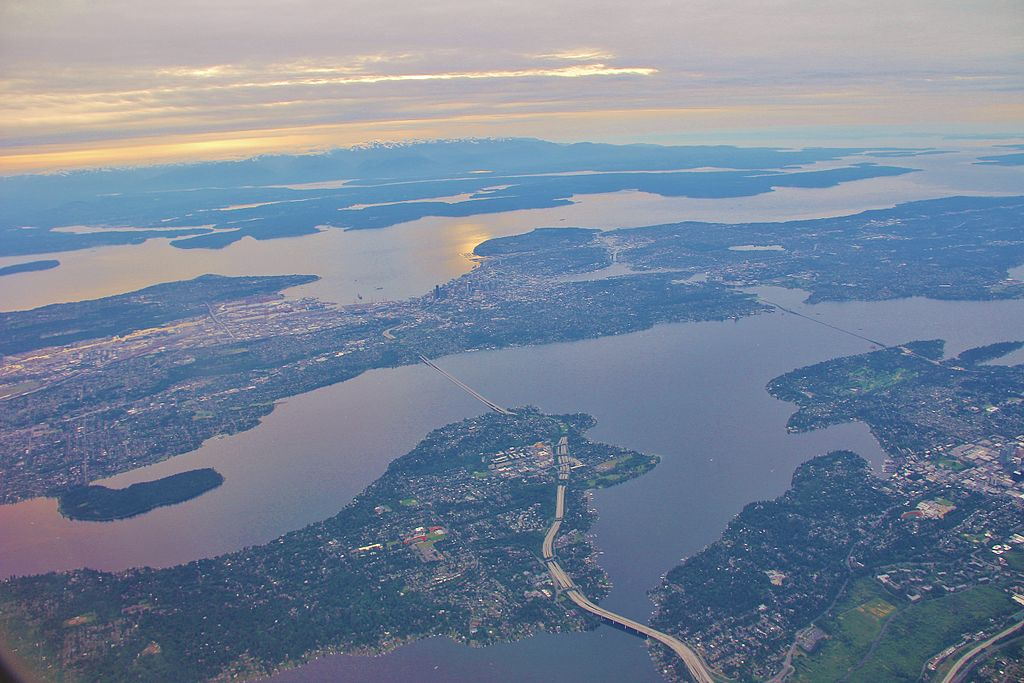
\includegraphics{images/seattle-aerial-wikicommons.jpg}

}

\caption{Central Puget Sound \textbar{} Photo courtesy of
\hyperref[0]{Clemens Vasters from Viersen, Germany}, \hyperref[0]{CC BY
2.0}, via Wikimedia Commons}

\end{figure}%

\subsection{The Central Puget Sound
Region}\label{the-central-puget-sound-region}

The Puget Sound metropolitan region is one of North America's major
growth centers for people, jobs, and housing. Between 2010 and 2023, the
central Puget Sound's four-county region (King, Snohomish, Pierce, and
Kitsap counties) added more residents and housing units than the rest of
Washington state combined.\footnote{The source of these statistics are
  the author's analysis of postcensial estimates by the Washington State
  Office of Financial Management. The central Puget Sound population
  grew by 414,400 people between 2010 and 2023, while the rest of the
  state's population grew by 84,300 people. During the same period,
  276,177 housing units were added in the this region, while 179,786
  units were created elsewhere in the state.} According to forecasts by
the Puget Sound Regional Council, the region's population is expected to
grow to 5.8 million people living within 2.8 million households by
2050.(Puget Sound Regional Council, 2018)

One challenge that the central Puget Sound region faces is high, rising
housing costs. The Puget Sound Regional Council's \emph{Housing
Stability Strategy: 2023 Monitoring Report} provides several sobering
statistics about the region's housing costs. According to the report,
during the decade between 2010 and 2020, the region added only one
housing unit for every three new people that were born or moved there.
By 2023, the annual income required to purchase the area's median priced
home was \$160,000.\footnote{This estimate includes three of the four
  central Puget Sound counties: King, Pierce, and Snohomish.} Between
July 2015 and July 2023, the median rent cost increased by 50\%.(Puget
Sound Regional Council, 2023)

\subsection{Transit-Oriented
Development}\label{transit-oriented-development}

Transit-oriented development (TOD) is a strategy of building homes at or
near public transportation stops and stations. In the United States,
this strategy has had a complicated record---often leading to increased
property values while simultaneously lowering household travel costs and
reducing reliance on personal vehicles.(Lund, 2006) TOD often raises
concerns about the displacement of low-income residents and small
businesses, leading some local and regional governments to include
affordability requirements in their TOD programs.(Dawkins \& Moeckel,
2016)

While these concerns are valid, there is not an obvious, better
alternative to TOD. Sharp increases in sprawling, low-density
residential and commercial development in Washington during 1980s
resulted in many unintended consequences, including ecological
disruption, traffic congestion, urban disinvestment, and loss of
agricultural lands. This led the Washington State Legislature to adopt
the Growth Management Act (GMA), a law requiring cities and counties to
plan to accommodate growth within designated areas (urban growth areas
or UGAs).(Trohimovich, 2002) Many of the GMA's goals are highly aligned
with TOD---particularly the first four goals of the law.\footnote{The
  first four goals of
  \href{https://app.leg.wa.gov/rcw/default.aspx?cite=36.70a.020}{\emph{RCW
  36.70A.020 Planning goals}} are:

  \begin{quote}
  (1) Urban growth. Encourage development in urban areas where adequate
  public facilities and services exist or can be provided in an
  efficient manner. (2) Reduce sprawl. Reduce the inappropriate
  conversion of undeveloped land into sprawling, low-density
  development. (3) Transportation. Encourage efficient multimodal
  transportation systems that will reduce greenhouse gas emissions and
  per capita vehicle miles traveled, and are based on regional
  priorities and coordinated with county and city comprehensive plans.
  (4) Housing. Plan for and accommodate housing affordable to all
  economic segments of the population of this state, promote a variety
  of residential densities and housing types, and encourage preservation
  of existing housing stock.
  \end{quote}}

\section{Data \& Methods}\label{sec-data-methods}

\section{Results}\label{results}

\section{Discussion}\label{discussion}

\section{Conclusion}\label{conclusion}

\section*{References}\label{references}
\addcontentsline{toc}{section}{References}

\phantomsection\label{refs}
\begin{CSLReferences}{1}{0}
\vspace{1em}

\bibitem[\citeproctext]{ref-dawkins2016}
Dawkins, C. J., \& Moeckel, R. (2016). Transit-induced gentrification:
Who will stay, and who will go? \emph{Housing Policy Debate}, \emph{26},
801--818. \url{https://doi.org/10.1080/10511482.2016.1138986}

\bibitem[\citeproctext]{ref-lund2006}
Lund, H. (2006). Reasons for living in a transit-oriented development,
and associated transit use. \emph{Journal of the American Planning
Association}, \emph{72}, 357--366.
\url{https://doi.org/10.1080/01944360608976757}

\bibitem[\citeproctext]{ref-pugetsoundregionalcouncil2018}
Puget Sound Regional Council. (2018). \emph{Draft 2050 forecast of
people and jobs}. Retrieved from \url{https://www.psrc.org/media/1749}

\bibitem[\citeproctext]{ref-pugetsoundregionalcouncil2023}
Puget Sound Regional Council. (2023). \emph{Regional housing strategy:
2023 monitoring report}. Retrieved from
\url{https://www.psrc.org/sites/default/files/2023-11/reg-housing-strategy-monitoring-rpt-2023.pdf}

\bibitem[\citeproctext]{ref-pugetsoundregionalcouncil2024}
Puget Sound Regional Council. (2024, January). Community and
transit-oriented housing development bill 2024: An interactive web map.
Retrieved from \url{https://arcg.is/0SSvK10}

\bibitem[\citeproctext]{ref-trohimovich2002}
Trohimovich, T. (2002). The growth management act (GMA) after more than
10 years: Another look \& a response to criticisms. \emph{Growth}.
Retrieved from
\url{http://www.futurewise.org/assets/resources/GMA_another_look.pdf}

\bibitem[\citeproctext]{ref-urbaninstitute}
Urban Institute. (2023). Urban institute puget sound zoning atlas.

\end{CSLReferences}



\end{document}
